\documentclass[12pt, oneside]{article}

\usepackage[letterpaper, scale=0.89, centering]{geometry}
\usepackage{fancyhdr}
\setlength{\parindent}{0em}
\setlength{\parskip}{1em}

\pagestyle{fancy}
\fancyhf{}
\renewcommand{\headrulewidth}{0pt}
\rfoot{\href{https://creativecommons.org/licenses/by-nc-sa/2.0/}{CC BY-NC-SA 2.0} Version \today~(\thepage)}

\usepackage{amssymb,amsmath,pifont,amsfonts,comment,enumerate,enumitem}
\usepackage{currfile,xstring,hyperref,tabularx,graphicx,wasysym}
\usepackage[labelformat=empty]{caption}
\usepackage[dvipsnames,table]{xcolor}
\usepackage{multicol,multirow,array,listings,tabularx,lastpage,textcomp,booktabs}

\lstnewenvironment{algorithm}[1][] {   
    \lstset{ mathescape=true,
        frame=tB,
        numbers=left, 
        numberstyle=\tiny,
        basicstyle=\rmfamily\scriptsize, 
        keywordstyle=\color{black}\bfseries,
        keywords={,procedure, div, for, to, input, output, return, datatype, function, in, if, else, foreach, while, begin, end, }
        numbers=left,
        xleftmargin=.04\textwidth,
        #1
    }
}
{}
\lstnewenvironment{java}[1][]
{   
    \lstset{
        language=java,
        mathescape=true,
        frame=tB,
        numbers=left, 
        numberstyle=\tiny,
        basicstyle=\ttfamily\scriptsize, 
        keywordstyle=\color{black}\bfseries,
        keywords={, int, double, for, return, if, else, while, }
        numbers=left,
        xleftmargin=.04\textwidth,
        #1
    }
}
{}

\newcommand\abs[1]{\lvert~#1~\rvert}
\newcommand{\st}{\mid}

\newcommand{\A}[0]{\texttt{A}}
\newcommand{\C}[0]{\texttt{C}}
\newcommand{\G}[0]{\texttt{G}}
\newcommand{\U}[0]{\texttt{U}}

\newcommand{\cmark}{\ding{51}}
\newcommand{\xmark}{\ding{55}}
 
\begin{document}
\begin{flushright}
    \StrBefore{\currfilename}{.}
\end{flushright} 
\section*{Monday May 23}




Recall definition:  $A$ is  {\bf  mapping  reducible to} $B$  means there is a computable function 
$f : \Sigma^* \to \Sigma^*$ such that {\it for all} strings  $x$ in $\Sigma^*$, 
\[
x  \in  A \qquad \qquad \text{if and  only  if} \qquad \qquad f(x) \in B.
\]
Notation:  when $A$  is mapping reducible to $B$, we write $A  \leq_m B$.

{\bf Theorem} (Sipser 5.23): If $A \leq_m B$ and $A$ is undecidable, then $B$ is undecidable.
    
{\bf Halting problem}
    \[
    HALT_{TM} = \{ \langle M, w \rangle \mid \text{$M$ is a  Turing machine, $w$ is  a string, and $M$ halts on $w$} \}
    \]

We will define a computable function that witnesses the mapping reduction $A_{TM} \leq_m HALT_{TM}$.

Using Theorem 5.23, we can then conclude that $HALT_{TM}$ is undecidable.

Define $F: \Sigma^* \to \Sigma^*$ by
    \[
    F(x) =  \begin{cases}
    const_{out} \qquad &\text{if  $x \neq \langle M,w \rangle$ for any Turing machine  $M$ and string  $w$ over the alphabet of $M$} \\
    \langle M', w \rangle \qquad &  \text{if $x = \langle M, w \rangle$ for some Turing machine  $M$ and string $w$ over the alphabet of $M$.}
    \end{cases}
    \]
    where $const_{out}  =  \langle  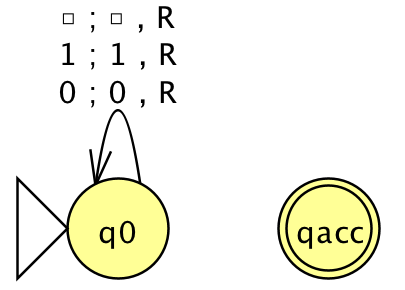
\includegraphics[width=1.5in]{Lect22TM1.png} ,  \varepsilon  \rangle$
    and  $M'$ is a Turing machine that computes like $M$ except, if the computation ever were to go to a  reject state,
    $M'$ loops instead.
    
    \vfill

    $F( \langle 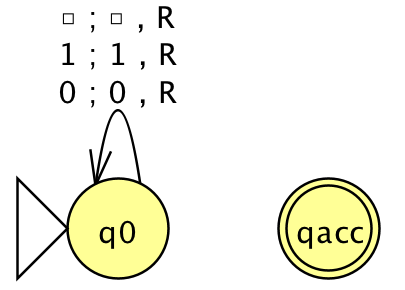
\includegraphics[width=1.5in]{Lect22TM1.png} ,  001  \rangle)$ =

    \vfill

    $F( \langle 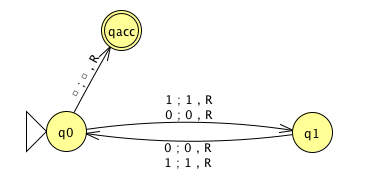
\includegraphics[width=2.5in]{Lect22TM2.png} ,  1  \rangle)$ =

    \vfill
    
    \newpage
    To use this function  to prove that $A_{TM} \leq_m HALT_{TM}$, we need  two claims:

    
    Claim (1): $F$ is computable \phantom{\hspace{2in}}
    
    \vfill

    Claim (2): for every  $x$,  $x \in  A_{TM}$ iff $F(x) \in HALT_{TM}$.  
    
    \vfill
   
    
\newpage
True or False: $\overline{A_{TM}} \leq_m \overline{HALT_{TM}}$

\vfill

True or False: $HALT_{TM} \leq_m A_{TM}$.

\vfill

\newpage     
\newpage
\subsection*{Review: Week 9 Monday}


Recall: Review quizzes based on class material are assigned each day. 
These quizzes will help you track and confirm your understanding of the concepts and examples 
we work in class. Quizzes can be submitted on Gradescope as many times (with no penalty) as 
you like until the quiz deadline: the three quizzes each week are all due on Friday (with no penalty 
late submission open until Sunday).

Please complete the review quiz questions on \href{http://gradescope.com}{Gradescope} about 
mapping reductions.


\newpage
\subsection*{Wednesday May 25}





Recall:  $A$ is  {\bf  mapping  reducible to} $B$, written $A \leq_m B$,  means there is a computable function 
$f : \Sigma^* \to \Sigma^*$ such that {\it for all} strings  $x$ in $\Sigma^*$, 
\[
x  \in  A \qquad \qquad \text{if and  only  if} \qquad \qquad f(x) \in B.
\]



{\bf Theorem} (Sipser 5.28): If $A \leq_m B$ and $B$ is recognizable, then $A$ is recognizable.

{\bf Proof}: 


\vfill


{\bf Corollary}: If  $A \leq_m B$ and $A$ is unrecognizable, then $B$ is unrecognizable.


\vfill



{\it Strategy}:  

(i) To prove that a  recognizable language $R$ is undecidable, prove that $A_{TM} \leq_m R$.


(ii) To prove that a co-recognizable language $U$ is undecidable, prove that $\overline{A_{TM}} \leq_m U$,
 i.e. that $A_{TM} \leq_m \overline{U}$.

\newpage

\[
E_{TM} = \{ \langle M \rangle \mid \text{$M$ is a Turing machine and $L(M) = \emptyset$} \}
\]

Example  string in  $E_{TM}$ is \underline{\phantom{\hspace{1.6in}}} .
Example  string not  in  $E_{TM}$ is \underline{\phantom{\hspace{1.6in}}} .

$E_{TM}$ is ~~decidable /  undecidable~~ and ~~recognizable /  unrecognizable~~.

$\overline{E_{TM}}$ is ~~decidable /  undecidable~~ and ~~recognizable /  unrecognizable~~.


{\bf Claim}: $\underline{\phantom{\hspace{1.6in}}}  \leq_m \overline{E_{TM}}$.

{\bf Proof}: Need computable function  $F: \Sigma^* \to \Sigma^*$  such that  $x \in A_{TM}$ iff $F(x)  \notin  E_{TM}$.
Define
\begin{quote}
$F =  ``$ On input $x$,
\begin{itemize}
\item[1.] Type-check whether  $x = \langle M, w \rangle$ for some TM $M$ and string $w$.   If so, move to step 2; if  not, output 
\item[2.] Construct the following machine $M'_x$:
\vspace{50pt}
\item[3.] Output $\langle M'_x \rangle$."
\end{itemize}
\end{quote}

Verifying correctness:
\begin{center}
\begin{tabular}{|c|c|}
\hline
Input string &  Output string \\
\hline
$\langle M, w \rangle$ where  $w \in L(M)$ & \phantom{\hspace{4in}} \\
& \\
$\langle M, w \rangle$ where $w \notin L(M)$ & \\
&\\
$x$ not encoding any pair of  TM and string   &  \\
\hline
\end{tabular}
\end{center}

\newpage
\[
EQ_{TM} = \{ \langle M, M' \rangle \mid \text{$M$ and $M'$ are both Turing machines and $L(M) =L(M')$} \}
\]

Example  string in  $EQ_{TM}$ is \underline{\phantom{\hspace{1.5in}}} .
Example  string not  in  $EQ_{TM}$ is \underline{\phantom{\hspace{1.5in}}} .

$EQ_{TM}$ is ~~decidable /  undecidable~~ and ~~recognizable /  unrecognizable~~.

$\overline{EQ_{TM}}$ is ~~decidable /  undecidable~~ and ~~recognizable /  unrecognizable~~.

To  prove, show that  $\underline{\phantom{\hspace{1.6in}}}  \leq_m EQ_{TM}$
and that $\underline{\phantom{\hspace{1.6in}}}  \leq_m \overline{EQ_{TM}}$.


\vfill

Verifying correctness:
\begin{center}
\begin{tabular}{|c|c|}
\hline
Input string &  Output string \\
\hline
$\langle M, w \rangle$ where  $M$ halts on $w$ & \phantom{\hspace{4in}} \\
& \\
$\langle M, w \rangle$ where $M$ loops on $w$ & \\
&\\
$x$ not encoding any pair of  TM and string   &  \\
\hline
\end{tabular}
\end{center}

\vfill

\newpage 
\subsection*{Review: Week 9 Wednesday}

Please complete the review quiz questions on \href{http://gradescope.com}{Gradescope} about 
mapping reductions.

{\bf Pre class reading for next time}: Introduction to Chapter 7.



\newpage
\subsection*{Friday May 27}




In practice, computers (and Turing machines) don't have infinite tape, 
and we can't afford to wait unboundedly long for an answer.
``Decidable" isn't good enough - we want ``Efficiently decidable".

For a given algorithm working on a given input, how long do we need to wait for an answer? 
How does the running time depend on the input in the worst-case? average-case? 
We expect to have to spend more time on computations with larger inputs.


A language is {\bf recognizable} if \underline{\phantom{\hspace{4.5in}}}

A language is {\bf decidable} if \underline{\phantom{\hspace{4.7in}}}

A language is {\bf efficiently  decidable} if \underline{\phantom{\hspace{4in}}}

A function is {\bf computable} if \underline{\phantom{\hspace{4.7in}}}

A function is {\bf efficiently computable} if \underline{\phantom{\hspace{4in}}}\\

\vfill

Definition  (Sipser 7.1): For  $M$ a deterministic decider, its {\bf running time} is the function  $f: \mathbb{N} \to \mathbb{N}$
given  by
\[
f(n) =  \text{max number of  steps $M$ takes before halting, over all inputs  of length $n$}
\]

Definition (Sipser 7.7): For each function $t(n)$, the {\bf time complexity class}  $TIME(t(n))$, is defined  by
\[
TIME( t(n)) = \{ L \mid \text{$L$ is decidable by  a Turing machine with running time in  $O(t(n))$} \}
\]

An example of an element of  $TIME(  1  )$ is 

An example of an element of  $TIME(  n  )$ is 


Note: $TIME( 1) \subseteq TIME (n)  \subseteq TIME(n^2)$

\vfill

Definition (Sipser 7.12) : $P$ is the class of languages that  are decidable in polynomial time on 
a deterministic 1-tape  Turing  machine
\[
P  =  \bigcup_k TIME(n^k)
\]

{\it Compare to exponential time: brute-force search.}


Theorem (Sipser 7.8): Let $t(n)$ be a  function with  $t(n)  \geq n$.  Then every $t(n)$ time deterministic 
multitape Turing machine has an equivalent $O(t^2(n))$ time deterministic 1-tape Turing machine.



\newpage


Definition (Sipser  7.9): For $N$ a nodeterministic decider.  
The {\bf running time} of $N$ is the function $f: \mathbb{N} \to \mathbb{N}$ given  by
\[
f(n) =  \text{max number of  steps $N$ takes on  any branch before halting, over all inputs  of length $n$}
\]

Definition (Sipser 7.21): For each function $t(n)$, the {\bf nondeterministic time complexity class}  
$NTIME(t(n))$, is defined  by
\[
NTIME( t(n)) = \{ L \mid \text{$L$ is decidable by a nondeterministic Turing machine with running time in $O(t(n))$} \}
\]
\[
NP = \bigcup_k NTIME(n^k)
\]


{\bf True} or {\bf False}: $TIME(n^2) \subseteq NTIME(n^2)$

\vfill

{\bf True} or {\bf False}: $NTIME(n^2) \subseteq DTIME(n^2)$

\vfill

{\bf Examples in $P$ }

{\it Can't use nondeterminism; Can use multiple tapes; Often need to be “more clever” than naïve / brute force approach}
\[
    PATH = \{\langle G,s,t\rangle \mid \textrm{$G$ is digraph with $n$ nodes there is path from s to t}\}
\]
Use breadth first search to show in $P$
\[
    RELPRIME = \{ \langle x,y\rangle \mid \textrm{$x$ and $y$ are relatively prime integers}\}
\]
Use Euclidean Algorithm to show in $P$
\[
    L(G) = \{w \mid \textrm{$w$ is generated by $G$}\} 
\]
(where $G$ is a context-free grammar). Use dynamic programming to show in $P$.

\vfill
{\bf Examples in $NP$}

{\it ``Verifiable" i.e. NP, Can be decided by a nondeterministic TM in polynomial time,
best known deterministic solution may be brute-force, 
solution can be verified by a deterministic TM in polynomial time.}

\[
    HAMPATH = \{\langle G,s,t \rangle \mid \textrm{$G$ is digraph with $n$ nodes, there is path
from $s$ to $t$ that goes through every node exactly once}\}
\]
\[
    VERTEX-COVER = \{ \langle G,k\rangle \mid \textrm{$G$ is an undirected graph with $n$
nodes that has a $k$-node vertex cover}\}
\]
\[
    CLIQUE = \{ \langle G,k\rangle \mid \textrm{$G$ is an undirected graph with $n$ nodes that has a $k$-clique}\}
\]
\[
    SAT =\{ \langle X \rangle \mid \textrm{$X$ is a satisfiable Boolean formula with $n$ variables}\}
\]

\newpage 
\newpage
\subsection*{Review: Week 9 Friday}


Please complete the review quiz questions on \href{http://gradescope.com}{Gradescope} about 
TBD

{\bf Pre class reading for next time}: Skim Chapter 7.

In observance of Memorial Day, there will be no lecture or discussion section on Monday.

\end{document}